\section{Methods used}


	\subsection{Central truncation}

		\begin{frame}{Central Truncation}

			\begin{itemize}
				\item The most common and straightforward approach used in practice to handle
				inputs exceeding the context size.
				\item Generally, sequences are truncated from the end before processing.
				\item Some studies show that truncating the middle produced better results
				\citep{sun2019fine, worsham-kalita-2018-genre}.
				\item We keep a fraction of the tokens from the head and the tail, i.e. truncate
				the middle.
				\item Hyperparameter $head\_size \in [0, 1]$ controls the fraction of tokens taken
				from the head.
			\end{itemize}

		\end{frame}


	\subsection{Document Skimming}

		\begin{frame}{Document Skimming}

			\begin{itemize}
				\item This approach is inspired by the fast reading technique "skimming".
				\item It involves reading while skipping some parts of the text for efficiency.
				\item Reader attempts to skip the redundant or irrelevant parts.
			\end{itemize}

			\vskip .5cm

			\begin{figure}
				\centering
				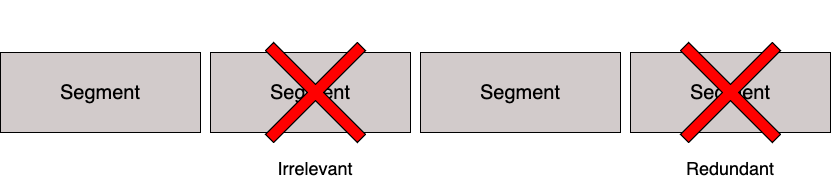
\includegraphics[width=\textwidth]{Images/skim.png}
			\end{figure}

		\end{frame}

		\begin{frame}{Document Skimming (contd.)}

			\begin{itemize}
				\item We uniformly sample the text segments to fill the LLM's context size.
				\item Each segment has equal probability of being selected since we do not know
				which parts are important.
				\item This ensures we capture details from every part of the document.
				\item We also experiment with removing similar segments before and after sampling.
			\end{itemize}

			\vskip .5cm

			\begin{figure}
				\centering
				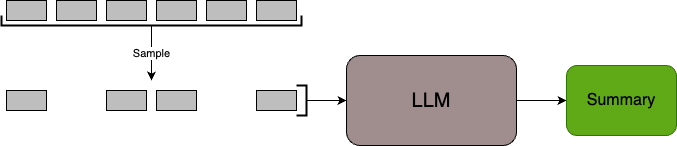
\includegraphics[width=\textwidth]{Images/doc-skim.png}
			\end{figure}

		\end{frame}


	\subsection{Summarization w/ Extraction}

		\begin{frame}{Summarization with Keyword Extraction}

			\begin{itemize}
				\item We use keywords from the document to select the most important segments.
				\item We use Latent Dirichlet Allocation (LDA) \citep{blei2003latent} with
				a single topic to extract keywords.
				\item Keywords are concatenated using a delimiter and embedded using a
				sentence transformer.
				\item Segments are scored by computing cosine similarity between keyword embedding
				and segment embeddings, also computed using the sentence transformer.
				\item Segments with the highest scores are chosen.
			\end{itemize}

		\end{frame}
